\documentclass[reqno,a4paper,12pt]{amsart}

\usepackage{amsmath,amssymb,amsthm,geometry,xcolor,soul,graphicx}
%\usepackage{array}
\usepackage{float} % 在tcolorbox中添加table (由于tcolorbox已经是一个box,因此不能直接加table)
\usepackage{titlesec}
%\usepackage{enumitem}
\usepackage{enumerate}
\usepackage{lipsum}
\usepackage{listings}
\allowdisplaybreaks[4] %align公式跨页
\RequirePackage[most]{tcolorbox}
\usepackage{braket}
%\usepackage{esint} %$\varoiint$ (带圈的二重积分)
%\usepackage[colorlinks,linkcolor=red]{hyperref} %\url{}超链接
\usepackage[scheme=plain,linespread=1,punct=CCT]{ctex}% Chinese support, single line space, narrow-version SBC case punctuations
\setCJKfamilyfont{zhsong}[AutoFakeBold={2.17}]{SimSong-Regular}
\renewcommand{\songti}{\CJKfamily{zhsong}}
%\usepackage{xeCJK}
%\setCJKmainfont{Kai}
\geometry{left=0.7in, right=0.7in, top=1in, bottom=1in}

\renewcommand{\baselinestretch}{1.3}

\title{固体物理第十次作业}
\author{董建宇 ~~ 2019511017}

\begin{document}

\maketitle

\begin{enumerate}[1.]
\item \textbf{(15.1) $\ddagger$ Nearly Free Electron Model}\\
Consider an electron in a weak periodic potential in one dimension $V(x) = V(x+a)$. Write the periodic potential as 
\[
	V(x) = \sum_{G} e^{iGx} V_G
\]
where the sum is over the reciprocal lattice $G = 2\pi n/a$, and $V_G^* = V_{-G}$ assures that the potential $V(x)$ is real. \\
(a) Explain why for $k$ near to a Brillouin zone boundary (such as $k$ near $\pi/a$) the electron wave function should be taken to be 
\[
	\psi = Ae^{ikx} + Be^{i(k+G)x}
\]
where $G$ is a reciprocal lattice vector such that $\vert k \vert$ is close to $\vert k+G \vert$. \\
(b) For an electron of mass $m$ with $k$ exactly at a zone boundary, use the above form of the wave-function to show that the eigenenergies at this wave vector are 
\[
	E = \frac{\hbar^2k^2}{2m} + V_0 \pm \vert V_G \vert
\]
where $G$ is chosen so $\vert k \vert = \vert k+G \vert$. \\
$\triangleright$ Give a qualitative explanation of why these two states are separated in energy by $2\vert V_G \vert$. \\
$\triangleright$ Give a sketch (don't do a full calculate) of the energy as a function of $k$ in both the extended and the reduced zone schemes. \\
(c) *Now Consider $k$ close to, but not exactly at, the zone boundary. Give an expression for the energy $E(k)$ correct to order $(\delta k)^2$ where $\delta k$ is the wavecector difference from $k$ to the zone boundary wavevector. \\
$\triangleright$ Calculate the effective mass of an electron at this wavevector. 
\begin{tcolorbox}[breakable, colback = black!5!white, colframe = black]
\begin{enumerate}[(a)]
\item 在布里渊区边界处,由于波矢$k$与波矢$k+G$对应的能量十分接近,则需要利用兼并微扰理论求解,两个基矢分别为:$\ket{k}$与$\ket{k+G}$,则Hamiltonian本征态可以写为:
\[
	\ket{\psi} = A\ket{k} + \ket{k+G}.
\]
则坐标表象下波函数为:
\[
	\psi = \langle x \vert \psi \rangle = Ae^{ikx} + Be^{i(k+G)x}.
\]

\item $\triangleright$ 考虑电子波矢恰好在布里渊区边界处,则对应波矢$k$与波矢$k+G$的电子能量相等,等于$E_0 = \frac{\hbar^2k^2}{2m}+V_0$。但是由于势场的微扰,兼并能级被打开,也就是说两个态的能量出现差值$2\vert V_G \vert$。 \\
\textbf{定量计算:}在两个态$\ket{k}$与$\ket{k'} = \ket{k+G}$基底下,Hamiltonian可以写为:
\[
	H = \begin{pmatrix}
		\frac{\hbar^2(-\pi/a)^2}{2m} + V_0 & V_G^* \\
		V_G & \frac{\hbar^2(\pi/a)^2}{2m}+V_0
	\end{pmatrix}
\]
则Hamiltonian本征值满足:
\[
	\left\vert \begin{matrix}
		\frac{\hbar^2(-\pi/a)^2}{2m} + V_0 - E & V_G^* \\
		V_G & \frac{\hbar^2(\pi/a)^2}{2m} + V_0 - E
	\end{matrix} \right\vert = 0.
\]
则可以解得:
\[
	E = \frac{\hbar^2(\pi/a)^2}{2m} + V_0 \mp \vert V_G \vert = \frac{\hbar^2k^2}{2m} + V_0 \pm \vert V_G \vert.
\]
$\triangleright$ 色散关系如下图:\\
\begin{centering}
	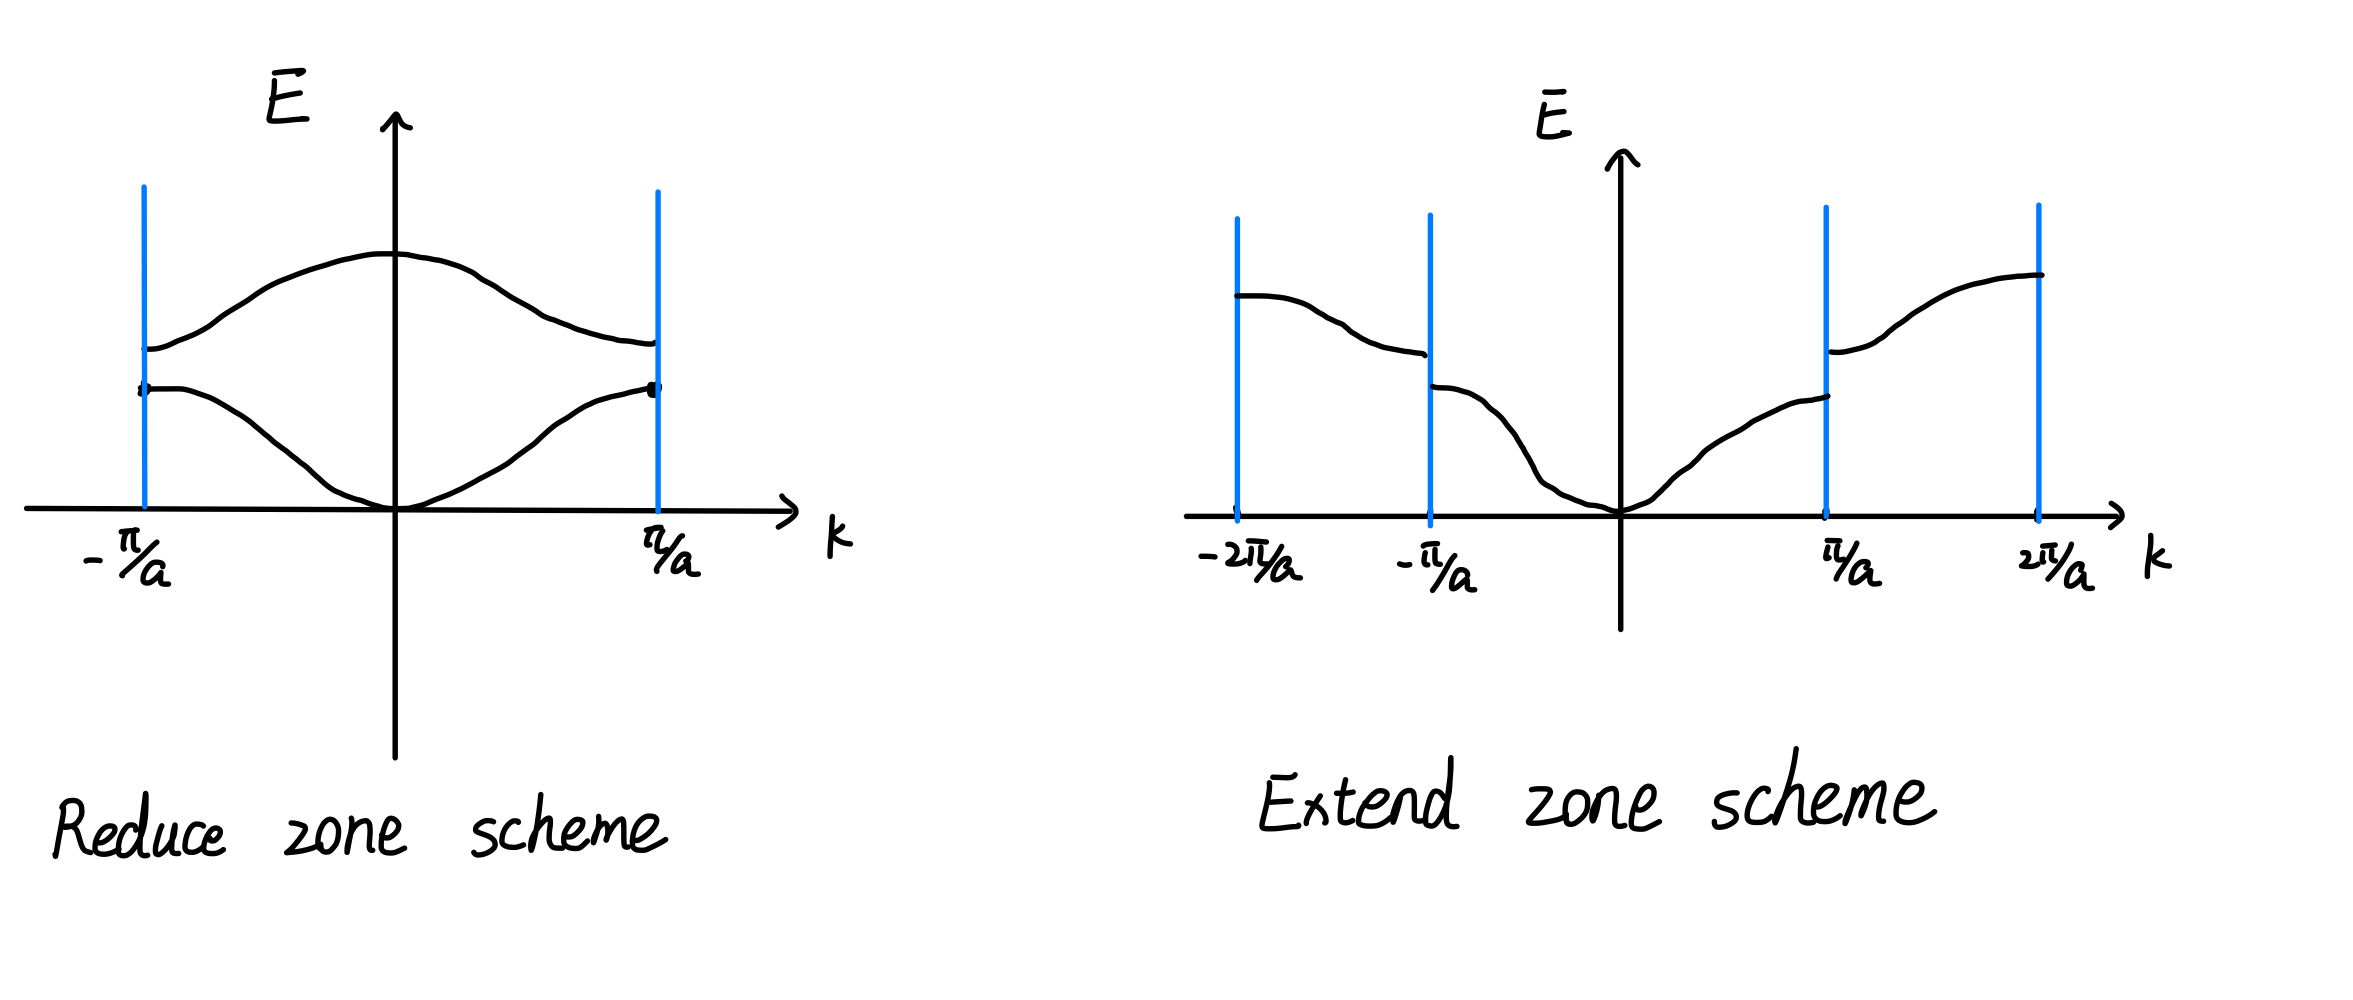
\includegraphics[scale = 0.17]{15.1.jpeg}
\end{centering}

\item 假设波矢为:$k=-\pi/a + \delta k$,则两波矢$k$与$k+G$为基底对应的Hamiltonian为:
\[
	H = \begin{pmatrix}
		\frac{\hbar^2}{2m}(-\pi/a+\delta k)^2 + V_0 & V_G^* \\
		V_G & \frac{\hbar^2}{2m}(\pi/a+\delta k)^2 + V_0
	\end{pmatrix}
\]
则本征值$E$满足:
\[
	\left\vert \begin{matrix}
		\frac{\hbar^2}{2m}((\pi/a)^2 + (\delta k)^2 - 2\pi(\delta k)/a) + V_0 - E & V_G^* \\
		V_G & \frac{\hbar^2}{2m}((\pi/a)^2 + (\delta k)^2 + 2\pi(\delta k)/a) + V_0 - E
	\end{matrix} \right\vert = 0
\]
可以解得:
\[
	E = \frac{\hbar^2}{2m}((\pi/a)^2 + (\delta k)^2) + V_0 \pm \sqrt{\vert V_G \vert^2 + \frac{\pi^2\hbar^4(\delta k)^2}{m^2a^2}}.
\]
当$\delta k \to 0$时,本征值近似得:
\[
	E = \frac{\pi^2\hbar^2}{2ma^2} + V_0 + \frac{\hbar^2(\delta k)^2}{2m} \pm \vert V_G \vert \left( 1 + \frac{\pi^2\hbar^4(\delta k)^2}{2\vert V_G \vert^2m^2a^2} \right)
\]
$\triangleright$ 有效质量满足:
\[
	\frac{\hbar^2(\delta k)^2}{2m^*} = \frac{\hbar^2(\delta k)^2}{2m} \pm \frac{\pi^2\hbar^4(\delta k)^2}{2\vert V_G \vert m^2a^2}.
\]
则可以解得:
\[
	m^* = \frac{\vert V_G \vert m^2a^2}{m\vert V_G \vert a^2 \pm \pi^2\hbar^2}
\]
\end{enumerate}
\end{tcolorbox}

\item \textbf{(15.3) Tight Binding Bloch Wavefunctions} \\
Analogous to the wavefunction introduced in Chapter 11, consider a tight-binding wave ansatz of the form 
\[
	\ket{\psi} = \sum_{R} e^{i\mathbf{k}\cdot\mathbf{R}} \ket{\mathbf{R}}
\]
where the sun is over the points $\mathbf{R}$ of a lattice, and $\ket{\mathbf{R}}$ is the ground-state wavefunction of an electron bound to a nucleus on site $\mathbf{R}$. In real space this ansatz can be expressed as 
\[
	\psi(\mathbf{r}) = \sum_{\mathbf{R}} e^{i\mathbf{k} \cdot \mathbf{R}} \varphi(\mathbf{r} - \mathbf{R}).
\]
Show that this wavefunction is of the form required by Bloch's theorem (i.e., show it is a modified plane wave).
\begin{tcolorbox}[breakable, colback = black!5!white, colframe = black]
该波函数可以写为:
\[
	\psi(\vec{r}) = e^{i\vec{k} \cdot \vec{r}} \sum_{\vec{R}} e^{-i\vec{k}\cdot(\vec{r}-\vec{R})} \varphi(\vec{r}-\vec{R}) = e^{i\vec{k}\cdot\vec{r}} u_{\vec{k}}(\vec{r}).
\]
接下来只需验证$u_{\vec{k}}(\vec{r})$的周期性。
\begin{align*}
	u_{\vec{k}}(\vec{r}+\vec{a}) =& \sum_{\vec{R}} e^{-i\vec{k}\cdot(\vec{r}+\vec{a}-\vec{R})} \varphi(\vec{r}+\vec{a}-\vec{R}) \\
	=& \sum_{\vec{R}' = \vec{R}-\vec{a}} e^{-i\vec{k}\cdot(\vec{r}-\vec{R}')} \varphi(\vec{r}-\vec{R}') \\
	=& \sum_{\vec{R}} e^{-i\vec{k}\cdot(\vec{r}-\vec{R})} \varphi(\vec{r}-\vec{R}) \\
	=& u_{\vec{k}}(\vec{r}).
\end{align*}
即这个波函数满足Bloch定理要求的形式。
\end{tcolorbox}

\item \textbf{(15.4) *Nearly Free Electrons in Two Dimensions} \\
Consider the nearly free electron model for a square lattice with lattice constant $a$. Suppose the periodic potential is given by 
\[
	V(x,y) = 2V_{10}[\cos(2\pi x/a) + \cos(2\pi y/a)] + 4V_{11}[\cos(2\pi x/a)\cos(2\pi y/a)]
\]
(a) Use the nearly free electron model to find the energies of states at wavevector $\mathbf{G} = (\pi/a,0)$. \\
(b) Calculate the energies of the states at wavevector $\mathbf{G} = (\pi/a,\pi/a)$. (Hint: You should write down a 4 by 4 secular determinant, which looks difficult, but actually factors nicely. Make use of adding together rows or columns of the determinant before trying to evaluate it!)
\begin{tcolorbox}[breakable, colback = black!5!white, colframe = black]
\begin{enumerate}[(a)]
\item 注意到倒格矢为$\mathbf{G} = (\pi/a,0)$的波矢与$(0,\pm \pi/a)$的波矢不满足动量守恒的Laue公式,所以只需考虑一维情况,位于$(\pm \pi/a, 0)$处的两个态能量简并,需利用简并微扰理论计算,则能量为:
\[
	E = \frac{\hbar^2(\pi/a)^2}{2m} \pm \vert V_G \vert.
\]
其中,$\vert V_G \vert$为:
\[
	\vert V_G \vert = \left\vert \frac{1}{a^2} \int_{-a/2}^{a/2}\int_{-a/2}^{a/2} e^{i\pi x/a} V(x,y) e^{i\pi x/a} \,dx\,dy \right\vert = \vert V_{10} \vert.
\]
则能量为:
\[
	E = \frac{\hbar^2(\pi/a)^2}{2m} \pm \vert V_{10} \vert.
\]

\item 注意到倒格矢为$\mathbf{G} = (\pi/a,\pi/a)$的波与$(\pi/a,-\pi/a)$和$(-\pi/a,\pm\pi/a)$能量简并,且满足动量守恒$\vec{k}' - \vec{k} = \vec{G}$,则需要在四维基底$(\pm \pi/a, \pm \pi/a)$上展开Hamiltonian,可以计算:
\begin{align*}
	&\bra{(\pi/a,\pi/a)} \hat{H} \ket{(\pi/a,\pi/a)} = \frac{\hbar^22(\pi/a)^2}{2m} = \epsilon_0 \\
	&\bra{(\pi/a,\pi/a)} \hat{H} \ket{(\pi/a, -\pi/a)} = V_{10} \\
	&\bra{(\pi/a,\pi/a)} \hat{H} \ket{(-\pi/a,\pi/a)} = V_{10} \\
	&\bra{(\pi/a,\pi/a)} \hat{H} \ket{(-\pi/a,-\pi/a)} = V_{11} \\
	&\bra{(\pi/a,-\pi/a)} \hat{H} \ket{(-\pi/a,\pi/a)} = V_{11} \\
	&\bra{(\pi/a,-\pi/a)} \hat{H} \ket{(-\pi/a,-\pi/a)} = V_{10} \\
	&\bra{(-\pi/a,\pi/a)} \hat{H} \ket{(-\pi/a,-\pi/a)} = V_{10} 
\end{align*}
则矩阵为:
\[
	H = \begin{pmatrix}
		\epsilon_0 & V_{10} & V_{10} & V_{11} \\
		V_{10} & \epsilon_0 & V_{11} & V_{10} \\
		V_{10} & V_{11} & \epsilon_0 & V_{10} \\
		V_{11} & V_{10} & V_{10} & \epsilon_0
	\end{pmatrix}.
\]
特征值满足:
\[
	\left\vert \begin{matrix}
		\epsilon_0-E & V_{10} & V_{10} & V_{11} \\
		V_{10} & \epsilon_0-E & V_{11} & V_{10} \\
		V_{10} & V_{11} & \epsilon_0-E & V_{10} \\
		V_{11} & V_{10} & V_{10} & \epsilon_0-E
	\end{matrix} \right\vert = 0
\]
整理可得:
\[
	(\epsilon_0-E-V_{11})^2(\epsilon_0-E+V_{11}+2V_{10})(\epsilon_0-E+V_{11}-2V_{10}) = 0
\]
即对应倒格矢$\mathbf{G} = (\pi/a,\pi/a)$的能量为:
\begin{align*}
	E_1 =& E_2 = \frac{2\hbar^2(\pi/a)^2}{2m} - V_{11}, \\ 
	E_3 =& \frac{2\hbar^2(\pi/a)^2}{2m} + V_{11} + 2V_{10}, \\
	E_4 =& \frac{2\hbar^2(\pi/a)^2}{2m} + V_{11} - 2V_{10}.
\end{align*}
\end{enumerate}
\end{tcolorbox}

\item \textbf{(15.5) Decaying Waves} \\
As we saw in this chapter, in one dimension, a periodic potential opens a band gap such that there are no plane-wave eigennstates between energies $\epsilon_0(G/2) - \vert V_G \vert$ and $\epsilon_0(G/2) + \vert V_G \vert$ with $G$ a reciprocal lattice vector. However, at these forbidden energies, decaying (evanescent) waves still exist. Assume the form 
\[
	\psi(x) = e^{ikx - \kappa x}
\]
with $0<\kappa\leq k$ and $\kappa$ real. Find $\kappa$ as a function of energy for $k = G/2$. For what range of $V_G$ and $E$ is your result valid?
\begin{tcolorbox}[breakable, colback = black!5!white, colframe = black]
对于该形式的波,可令$k' = k+i\kappa$,则波函数可以写为:$\psi(x) = e^{ik'x}$,则对于布里渊区边界处的态的能量,满足:
\[
	\left\vert \begin{matrix}
		\frac{\hbar^2}{2m}(-G/2+i\kappa)^2 - E & V_G^* \\
		V_G & \frac{\hbar^2}{2m}(G/2+i\kappa)^2 - E
	\end{matrix}\right\vert = 0
\]
则可以解得:
\[
	E = \frac{\hbar^2}{2m}(G^2/4-\kappa^2) \pm \sqrt{\vert V_G \vert^2-\frac{\hbar^4\kappa^2G^2}{4m^2}}.
\]
则可以解得:
\[
	\kappa^2 = -\frac{2m}{\hbar^2}\left( E + \frac{\hbar^2G^2}{8m} \right) + \sqrt{\frac{m}{\hbar^2}\left( 2EG^2 + \frac{4m\vert V_G \vert^2}{\hbar^2} \right)}
\]
满足$\kappa^2>0$,可得:
\[
	mE\hbar^2G^4+4m^2(\vert V_G \vert^2-E^2) > \frac{\hbar^4G^4}{16}.
\]
即$\vert V_G \vert^2 > \left( E-\frac{\hbar G^2}{8m} \right)^2$
\end{tcolorbox}

\end{enumerate}

\end{document}